\documentclass[12pt,a4paper]{article}
\usepackage[T1]{fontenc}
\usepackage[utf8]{inputenc}
\usepackage[english]{babel}
\usepackage{tgschola}
\usepackage[scaled=0.94]{helvet}
\renewcommand{\familydefault}{\rmdefault}
\usepackage[a4paper,margin=2.5cm,headheight=15pt]{geometry}
\usepackage{xcolor,graphicx,float,booktabs,tabularx,array,enumitem,fancyhdr,titlesec,tocloft,pdflscape}
\usepackage[most]{tcolorbox}
\usepackage{csquotes,xurl,hyperref,cleveref}
\usepackage[backend=biber,style=ieee]{biblatex}
\addbibresource{documentation.bib}

\definecolor{PacBlue}{HTML}{1F3A5F}
\definecolor{SoftGray}{HTML}{F5F6F8}
\hypersetup{colorlinks=true,linkcolor=PacBlue,citecolor=PacBlue,urlcolor=PacBlue,
  pdftitle={Pac-Man AI -- Sprint 2 Documentation},pdfauthor={Pac-Man AI Team}}
\pagestyle{fancy}
\fancyhf{}
\lhead{\textsf{Pac-Man AI}}
\rhead{\textsf{Sprint 2 Documentation}}
\cfoot{\thepage}
\setlist[itemize]{leftmargin=1.5em,itemsep=0.2em}
\setlength{\parindent}{0pt}
\setlength{\parskip}{0.55em}
\setlength{\emergencystretch}{3em}
\titleformat{\section}{\Large\bfseries\sffamily\color{PacBlue}}{\thesection}{0.7em}{}
\titleformat{\subsection}{\large\bfseries\sffamily\color{PacBlue}}{\thesubsection}{0.7em}{}
\newtcolorbox{note}{colback=SoftGray,colframe=PacBlue,boxrule=0.5pt,arc=2pt,
  left=8pt,right=8pt,top=6pt,bottom=6pt}

\begin{document}

\pagenumbering{gobble}
\hypersetup{pageanchor=false}
\begin{titlepage}
  \centering
  \IfFileExists{images/utcn-logo.jpg}{\includegraphics[height=1.4cm]{images/utcn-logo.jpg}\par}{}
  {\Large\sffamily Technical University of Cluj-Napoca\par}
  \vspace{0.2cm}{\large Artificial Intelligence\par}
  \vspace{1.7cm}
  \IfFileExists{images/cover.png}{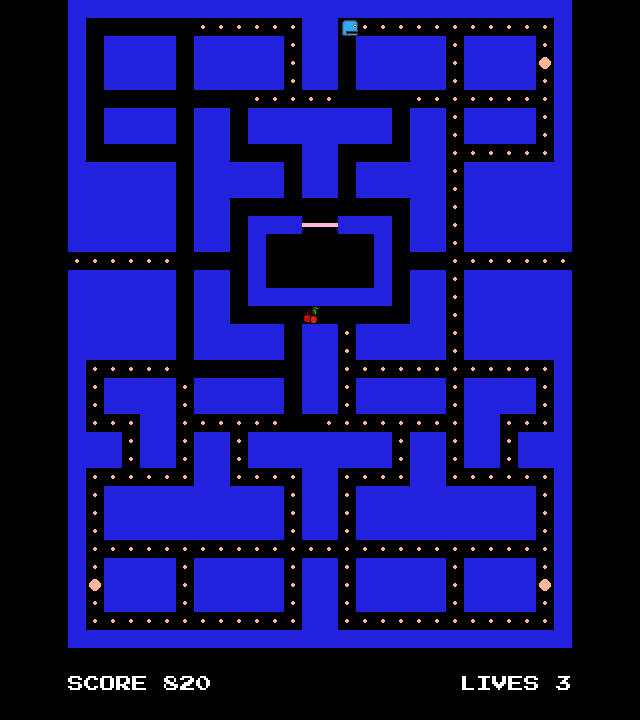
\includegraphics[width=0.62\linewidth]{images/cover.png}\par}{}
  \vspace{1cm}{\Huge\bfseries\color{PacBlue} Pac-Man AI\par}
  \vspace{0.4cm}{\Large Project Documentation -- Sprint 2\par}
  \vspace{0.8cm}{\large Four ghosts that hunt with search algorithms\par}
  \vfill
  {\large Ariana Daboc, Roxana Marginean, Diana Sighiartau\par}
  \vspace{0.5cm}Repository: \url{https://github.com/arianaDaboc/pacman}\par
  \vspace{0.3cm}\today
\end{titlepage}

\hypersetup{pageanchor=true}
\pagenumbering{roman}
\tableofcontents
\clearpage
\pagenumbering{arabic}

\section{Project Theme}
\label{sec:theme}

We wanted to build a Pac-Man game that feels familiar to anyone who has played the arcade original, without trying to reproduce every detail of it. The player guides Pac-Man through a maze, collects dots and energizers, and tries to clear the board. To keep the classic look, we used bright blue walls on a black background, together with pixel-style sprites and a matching font.

In Sprint 1, we focused on getting the basic game working from start to finish: loading the map, moving Pac-Man, keeping track of the score, and displaying the result. For Sprint 2, we added the four ghosts. Each ghost has its own way of choosing a destination, and uses a search algorithm to find a route there. The player can switch between the algorithms while the game is running. Pac-Man is still controlled with the keyboard; the autonomous Pac-Man is planned for Sprint 3.

We used drakzlin's free \enquote{20x20 Tileset} for the sprites and the Press Start 2P font by CodeMan38. The source and licence information for each asset is listed in \texttt{assets/ASSETS.md}. We also generated the sound effects specifically for this project using a small script.\cite{drakzlin2014tileset,pressstart2p}

\begin{figure}[H]
  \centering
  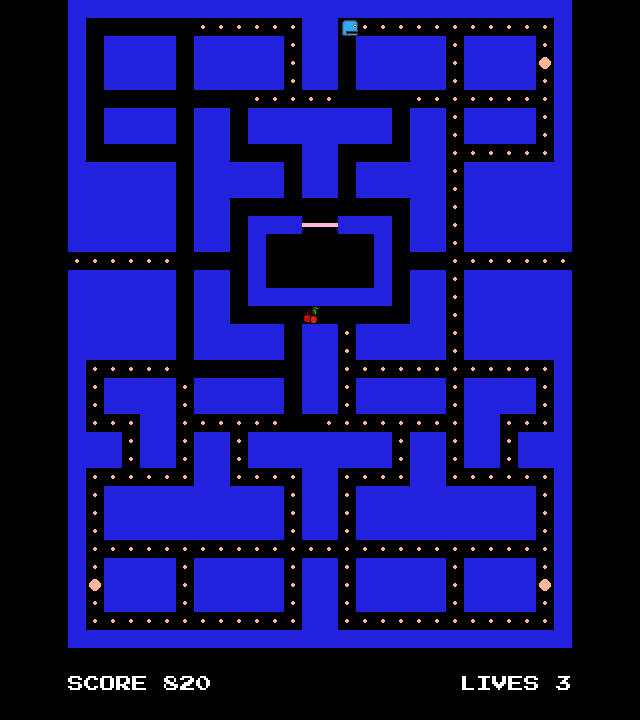
\includegraphics[width=0.62\linewidth]{images/gameplay.png}
  \caption{The game view.}
  \label{fig:gameplay}
\end{figure}

\section{Architecture}
\label{sec:architecture}

Figure~\ref{fig:classes} shows the classes and their connections at the end of Sprint 2. One thing we kept consistent is the separation between the game model and the graphical interface: classes such as \texttt{Maze}, \texttt{PacMan}, \texttt{Ghost}, \texttt{ModeTimer}, \texttt{Score}, the ghost personalities, and the search algorithms do not import Pygame. Pygame is used only by the classes in \texttt{view/} and by the game loop.

We made a few decisions that differ from the suggested architecture:
\begin{itemize}
  \item \textbf{We have not added a separate \texttt{GameState} class yet.} The rules that involve several characters, such as eating ghosts, being caught, and handling the timers, are currently managed by \texttt{Game}. They are handled in \texttt{update\_modes}, \texttt{target\_of}, and \texttt{check\_collisions}. For Sprint 3, the agents will need a state that they can copy and simulate, so we plan to move these methods into a \texttt{GameState} class then.
  \item \textbf{All ghosts share one \texttt{ModeTimer}.} The scatter/chase schedule and frightened time apply to all ghosts, so we keep track of them in a single object. It reports when a mode changes, and \texttt{Game} then updates the ghosts' modes and reverses their directions when needed. This keeps the reversal logic in one place.
  \item \textbf{Each ghost stores the information needed by the control panel.} After a search, a ghost remembers the length of its most recent path and how many nodes that search expanded. The control panel can display these values directly, without running the search a second time.
\end{itemize}

\begin{figure}[p]
  \centering
  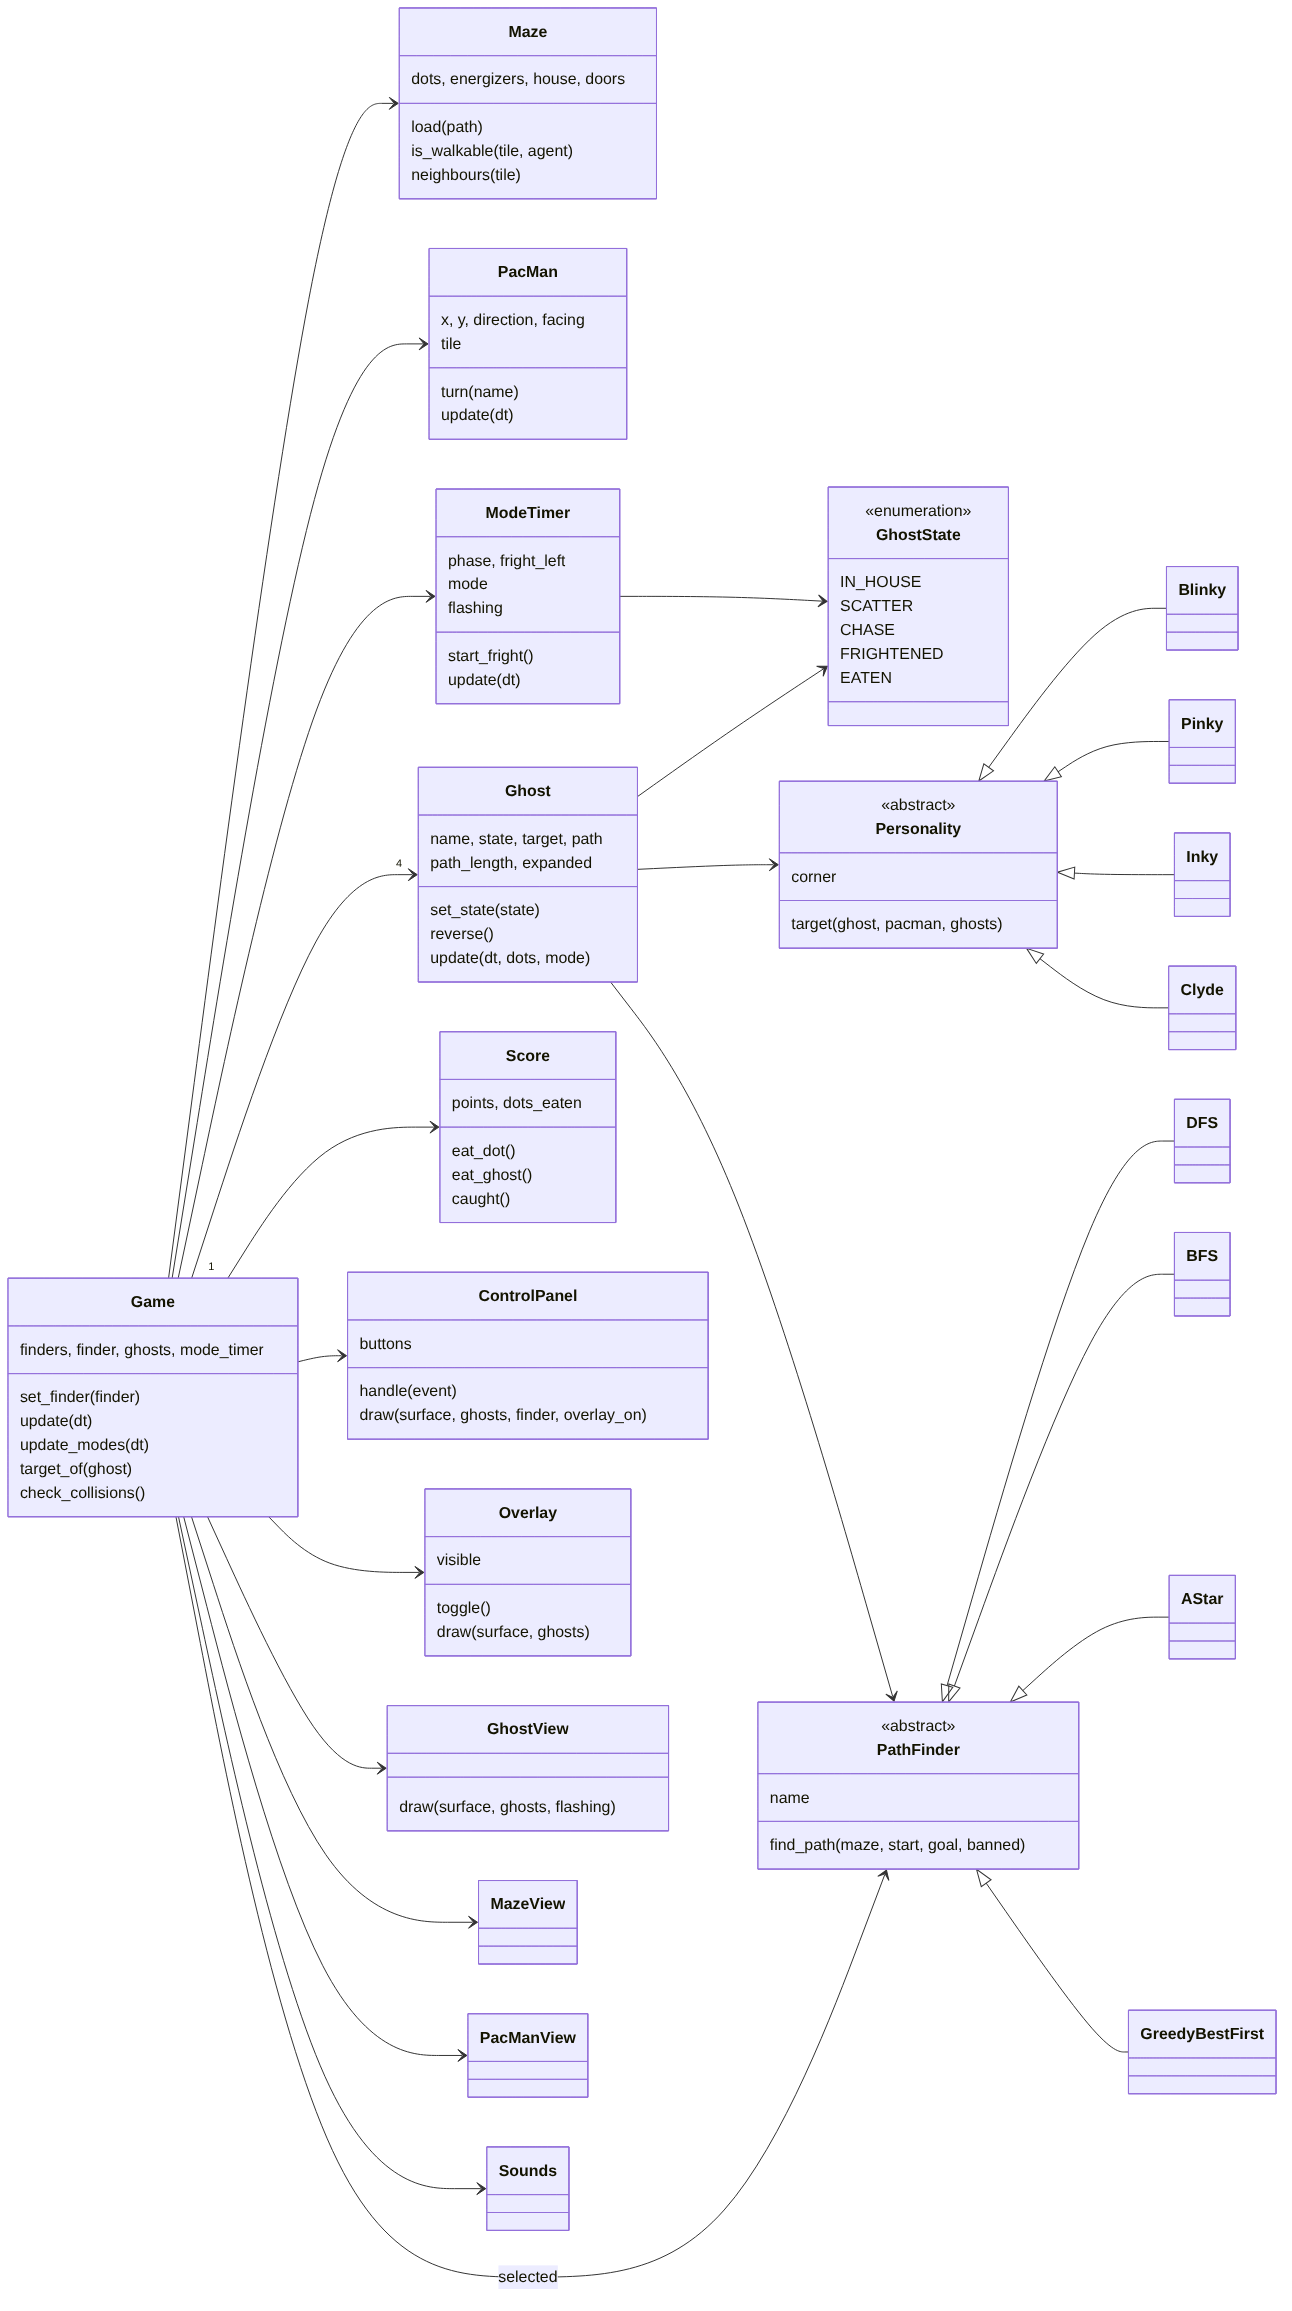
\includegraphics[height=0.86\textheight,keepaspectratio]{images/class-diagram.png}
  \caption{Class diagram of the code at the end of Sprint 2.}
  \label{fig:classes}
\end{figure}

\section{Maps}
\label{sec:maps}

The maze in \texttt{maps/classic.txt} is our own 28-by-36 layout. We kept it symmetrical from left to right so that both sides feel equally playable. The four energizers are placed near the corners, encouraging the player to use the outer corridors as well. A tunnel runs across the middle row, and the ghost house is in the centre of the board.

The map contains 307 dots, which is enough for the fruit to appear at both scoring thresholds. We also made the corridors connect back to the main paths instead of ending in dead ends wherever possible.

\begin{figure}[H]
  \centering
  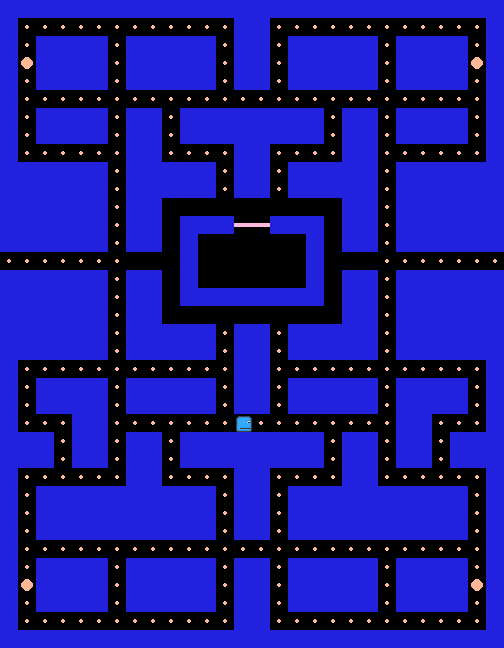
\includegraphics[width=0.48\linewidth]{images/map-default.png}
  \caption{The default maze.}
  \label{fig:map}
\end{figure}

\section{AI Design Decisions}
\label{sec:ai}

\setcounter{subsection}{2}
\subsection{Search Details}
\label{sec:search-details}

All four search algorithms (DFS, BFS, A* and greedy best-first) use the same \texttt{successors} helper in \texttt{search/path\_finder.py}. This helper returns the tiles a ghost can move to, always in the order up, left, down, right. It also applies the banned-move rule: on the first step, the tile directly behind the ghost is skipped, unless that tile is the only available way out. Since all four algorithms use the same helper, the main difference between them is how they order the frontier.

\paragraph{The ghost house.} A path that starts and ends in the corridors cannot pass through the ghost house or its door. These areas can only be used when a search starts or ends inside the house. This is needed, for example, when the eyes of an eaten ghost have to find their way back home.

\paragraph{A target tile that cannot be reached.} Pinky and Inky sometimes aim for tiles in front of Pac-Man that are actually walls or even outside the maze. The scatter corners on our map are also walls. Before a search begins, \texttt{closest\_walkable} replaces such a target with the corridor tile closest to it in a straight line, using Euclidean distance. If two or more tiles are equally close, the first one in reading order is selected. For example, Blinky's top-right corner, $(27,0)$, is replaced by $(26,1)$. The only target that is never changed is the ghost-house tile that the eyes return to.

\paragraph{The warp tunnel.} \texttt{Maze.neighbours} connects the left and right edges of each row, so moving through the tunnel costs the same as any other single step. All search algorithms can therefore use the tunnel without needing separate tunnel handling. The standard Manhattan distance does not account for this connection. When two tiles are on opposite sides of the tunnel, their actual distance can be much shorter than $|x_1-x_2|+|y_1-y_2|$. In that case, the plain Manhattan heuristic overestimates the distance, which means it is no longer admissible and A* may fail to return a shortest path.

For this reason, the A* implementation used in the game calculates the horizontal distance in both directions:
\[
  \min(|x_1-x_2|,\ w-|x_1-x_2|) + |y_1-y_2|,
\]
where $w$ is the width of the maze. This is the Manhattan distance adapted to a grid whose left and right edges connect. It does not overestimate the actual distance, so A* remains optimal. Greedy best-first still uses the plain Manhattan distance, as required by the project description. We also included A* with the plain heuristic in the experiment in Section~\ref{sec:results} to show the effect of the tunnel.

\paragraph{When a ghost runs a search.} A ghost starts a new search only when it reaches the centre of a tile and either its target has changed or it has used up its current path. If the player switches the algorithm in the control panel, all existing paths are cleared. The new algorithm is then used from the ghosts' next tile.

\section{Experiments and Results}
\label{sec:results}

\subsection{Search Comparison}
\label{sec:search-results}

We used the script \texttt{src/pacman/experiments/search\_comparison.py} to compare the four search algorithms, along with A* using the plain Manhattan distance. The tests were run on 30 fixed start/target pairs from \texttt{maps/classic.txt}. We selected three pairs by hand because their shortest paths go through the tunnel. The other 27 pairs were generated randomly from corridor tiles using a fixed seed. This way, every algorithm was tested on exactly the same pairs in each run.

Each search was timed 50 times, and we used the median time for the comparison. The raw results are available in \texttt{results/search\_comparison.csv}. Table~\ref{tab:search} summarises the measurements.

\begin{table}[H]
  \centering
  \caption{Search results for the same 30 start/target pairs. \enquote{Shortest paths} counts the pairs for which the algorithm found a path as short as BFS. The A* version used in the game has a tunnel-aware Manhattan distance; the plain variant is included only for comparison.}
  \label{tab:search}
  \begin{tabular}{lrrrr}
    \toprule
    Algorithm & Avg.\ path length & Shortest paths & Avg.\ expanded nodes & Avg.\ time (ms) \\
    \midrule
    DFS & 111.7 & 3/30 & 172.7 & 0.38 \\
    BFS & 21.1 & 30/30 & 155.7 & 0.33 \\
    A* & 21.1 & 30/30 & 42.7 & 0.12 \\
    A* (plain Manhattan) & 22.0 & 24/30 & 45.4 & 0.13 \\
    Greedy best-first & 24.0 & 18/30 & 27.0 & 0.07 \\
    \bottomrule
  \end{tabular}
\end{table}

\paragraph{Which algorithms find optimal paths?} BFS found a shortest path for all 30 pairs, which is what we expected because every move has the same cost and BFS explores tiles in order of their distance from the starting point. Our A* implementation also found a shortest path in all 30 cases. It did so while expanding fewer than a third of the nodes expanded by BFS on average: about 43 compared with 156.

\paragraph{What changes when A* uses the warp tunnel?} With the plain Manhattan heuristic, A* found a shortest path for only 24 of the 30 pairs. All six cases where it did not find a shortest path involved the tunnel; seven of the 30 pairs had a shortest route through it. For example, for the pair $(6,11)$ to $(21,17)$, BFS and our tunnel-aware A* both found a 19-tile route through the tunnel. A* with the plain heuristic returned a 27-tile route through the middle of the maze instead.

The plain Manhattan distance makes tiles near the tunnel appear farther from the target than they really are. As a result, the search reaches the target through the inner part of the maze first and stops there. This illustrates why the tunnel-aware distance is important for keeping A* optimal.

\paragraph{Which algorithm is fastest?} Greedy best-first expanded the fewest nodes (27 on average) and had the shortest execution time, followed by A* with an average of 43 expanded nodes. BFS and DFS each expanded more than 150 nodes on average, which is about a third of the maze. Greedy is fast, but its paths are not always the shortest: only 18 out of 30 matched the BFS path length, because the algorithm does not take the distance already travelled into account.

\paragraph{Why do DFS paths look unusual?} DFS follows one corridor as far as it can, trying directions in the fixed order and only going back when it reaches a dead end. It returns the first path it finds, rather than checking whether a shorter one exists. This is why its paths were, on average, about five times longer than BFS paths and often went through much of the maze. With the path overlay enabled, this is easy to notice: a DFS ghost may initially move away from Pac-Man before eventually turning back towards him.

\section{User Guide}
\label{sec:guide}

To run the game, first install \texttt{uv} by following the instructions on its official website. Then clone the repository and install the project dependencies. The command \texttt{uv sync} installs everything needed to run the game. The project requires Python 3.12 and Pygame.\cite{uv,pygame}

\begin{verbatim}
git clone https://github.com/arianaDaboc/pacman.git
cd pacman
uv sync
uv run pacman
\end{verbatim}

The game opens on a start screen. Press Enter or Space to begin. Use the arrow keys to move Pac-Man. If you press a direction that is not available straight away, the game keeps the input and tries to turn at the centre of the next tile, as long as that direction is open. Pac-Man stops when he reaches a wall, but he can travel through the horizontal warp tunnel. Press M to mute or unmute the sound. Closing the window exits the game.

You can also try the game using the smaller test map by running:

\begin{verbatim}
uv run pacman maps/small.txt --test
\end{verbatim}

With the \texttt{--test} option, the game checks only the map's file format. This means that a map that is too small for all the normal game rules can still be opened and played.

\begin{table}[H]
  \centering
  \caption{Controls.}
  \begin{tabular}{@{}ll@{}}
    \toprule
    \textbf{Key} & \textbf{Action} \\
    \midrule
    Enter or Space & Start the game; start a new game after a win or a game over \\
    Arrow keys & Steer Pac-Man \\
    1, 2, 3, 4 & Ghost search: DFS, BFS, A*, greedy best-first \\
    O & Show or hide the ghosts' paths and targets \\
    M & Mute or unmute the sound \\
    Close window & Quit \\
    \bottomrule
  \end{tabular}
\end{table}

Each dot is worth 10 points, and each energizer is worth 50 points. Fruit appears after 70 and 170 dots have been collected, stays on screen for nine seconds, and gives 100 points. After an energizer is collected, the ghosts turn blue for six seconds and flash during the final two seconds. Eating them gives 200, 400, 800, and 1600 points, respectively. If a ghost catches Pac-Man, the player loses a life and 500 points. The game is won when all dots and energizers have been collected, and it is lost when the last life is gone.

\paragraph{The control panel.} The panel to the right of the maze (Figure~\ref{fig:panel}) contains one button for each search algorithm. The player can click a button or press the corresponding number key to select an algorithm. All ghosts start using the selected algorithm from their next tile, and the active choice is highlighted.

Below the buttons, the panel displays each ghost's current state (house, scatter, chase, frightened, or eaten), as well as the length of its most recent path and the number of nodes expanded during its last search. Press O to show or hide the paths and target tiles on the maze. Each path is drawn in the colour of the ghost it belongs to.

\begin{figure}[H]
  \centering
  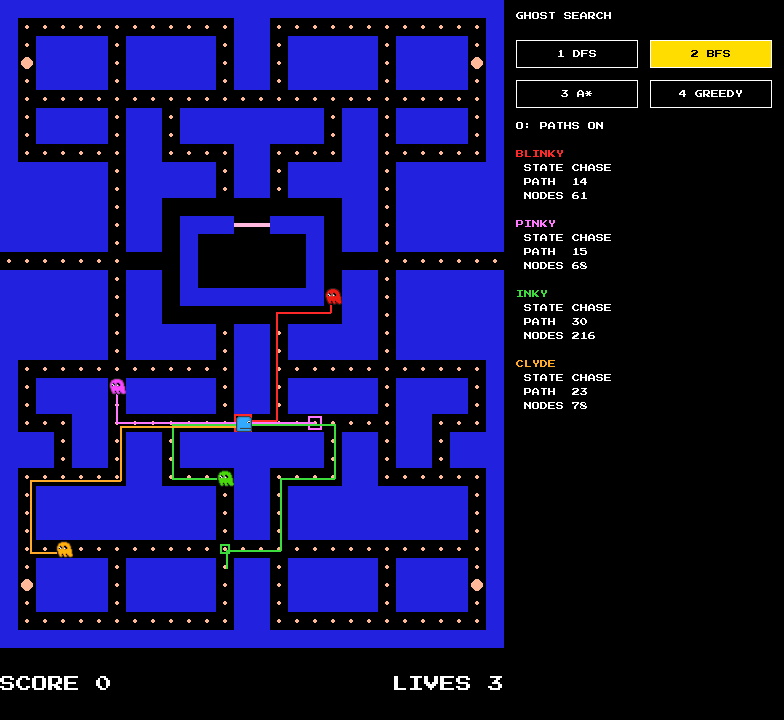
\includegraphics[width=0.75\linewidth]{images/control-panel.png}
  \caption{The game with the control panel and path overlay switched on.}
  \label{fig:panel}
\end{figure}

\begin{figure}[H]
  \centering
  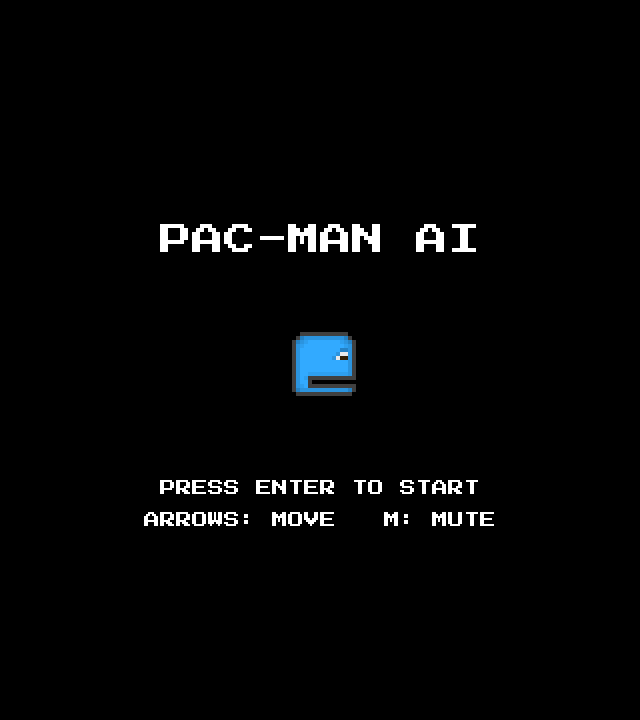
\includegraphics[width=0.42\linewidth]{images/start-screen.png}
  \caption{The start screen.}
  \label{fig:start}
\end{figure}

\section{Team}
\label{sec:team}

The work in Sprint 2 was shared across the three team members. The table below lists the main areas each person worked on, together with the user stories they were responsible for.

\begin{table}[H]
  \centering
  \caption{Main contributions and stories owned.}
  \begin{tabularx}{\textwidth}{@{}l X l@{}}
    \toprule
    \textbf{Member} & \textbf{Main contribution} & \textbf{Stories} \\
    \midrule
    Ariana Daboc & Project skeleton, map loading, README and documentation; DFS and BFS, the control panel and the search comparison & US1.0, US1.1, US1.6, US2.2, US2.6, US2.8 \\
    Roxana Marginean & Pac-Man movement and animation, start screen and sound; A* and the ghost states & US1.2, US1.5, US2.3, US2.5 \\
    Diana Sighiartau & Asset pack and theme, dots, fruit, score and win screen; the ghosts, their personalities and greedy best-first & US1.3, US1.4, US2.1, US2.4, US2.7 \\
    \bottomrule
  \end{tabularx}
\end{table}

\newpage
\nocite{pygame,uv}
\printbibliography[heading=bibintoc,title={References}]

\end{document}
